\documentclass[../main.tex]{subfiles}

\begin{document}

\begin{definition}
$A$ is a \textit{discrete valuation ring}\index{Discrete valuation ring} if $A$ is an integrally closed PID with a unique nonzero prime ideal. $k=A/m$, $m=(\pi)$, $\pi$ irreducible is unique up to $A^\times$, called the \textit{uniformizer}\index{Uniformizer}, $F=\Frac(A)=A[\frac{1}{\pi}]$
\end{definition}

\begin{proposition}
$A$ is a DVR, then $m^i-m^{i+1}=A^\times\pi^i$, $A^\times=A-m=\bigsqcup_{i\in\mathbb N}A^\times\pi^i$, $F^\times=\bigsqcup_{i\in\mathbb Z}A^\times\pi^i$
\begin{figure}[h!]
\centering
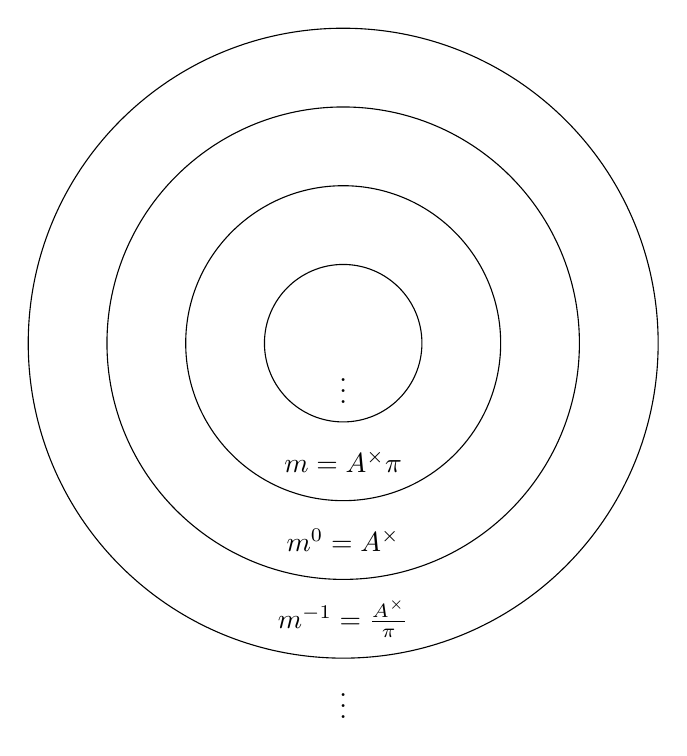
\begin{tikzpicture}
\foreach \r in {1,2,3,4}
{
\draw (0,0) circle (\r);
}
\node at (0,-0.5) {$\vdots$};
\node at (0,-1.5) {$m=A^\times\pi$};
\node at (0,-2.5) {$m^0=A^\times$};
\node at (0,-3.5) {$m^{-1}=\frac{A^\times}{\pi}$};
\node at (0,-4.5) {$\vdots$};
\end{tikzpicture}
\caption{Discrete Valuation Ring}\label{DVR}
\end{figure}
\end{proposition}

\begin{proposition}
$X$ is a compact Riemann surface, $F=\mathbb C(X)$, then $A=\{f\in F|f\text{ is defined at }x\}\subseteq F$ is a DVR
\end{proposition}

\begin{theorem}
$\sgn\disc(K/\mathbb Q)=(-1)^s$
\end{theorem}

\begin{proof}
$\disc(K/\mathbb Q)=\det(\Tr(\alpha_i\alpha_j))=(\det M)^2$, $M=(\sigma_i(\alpha_j))$, $\overline M=(\overline{\sigma_i(\alpha_j)})$, $\det\overline M=(-1)^s\det M$
\end{proof}

\begin{example}
\begin{itemize}
\item $\mathbb Z_{(p)}$ with $\pi=p$
\item $\mathbb C[t]_{(t-a)}$ with $\pi=t-a$
\item $\mathbb R[t]_{(t-c)}$ with $\pi=t-c$
\item $\mathbb F_p[t]_{(t-c)}$ with $\pi=t-c$
\end{itemize}
\end{example}

\begin{definition}
The additive valuation $\nu:F\to\mathbb Z\cup\{\infty\}$, $0\mapsto\infty$, $u\pi^i\mapsto i$ satisfies
\begin{enumerate}
\item $\nu(x)=\infty\Leftrightarrow x=0$
\item $\nu(xy)=\nu(x)+\nu(y)$
\item $\nu(x+y)\geq\min(\nu(x),\nu(u))$
\end{enumerate}
Any $\nu$ on $F$ satisfying 1.-3. knows $A$, i.e. $A=\{\nu\geq0\}$, $m=\{\nu>0\}$, $A^\times=\{\nu=0\}$
\end{definition}

\begin{definition}
$F$ is a field, a \textit{discrete valuation}\index{Discrete valuation} on $F$ is a function $F\to\mathbb R\cup\{\infty\}$ satisfying
\begin{enumerate}
\item $\nu(x)=\infty\Leftrightarrow x=0$
\item $\nu(xy)=\nu(x)+\nu(y)$
\item $\nu(x+y)\geq\min(\nu(x),\nu(u))$
\end{enumerate}
$\nu(F^\times)\subseteq\mathbb R$ is a lattice in $\mathbb R$. $\nu$ is normalized if $\nu(F^\times)=\mathbb Z$ is the standard lattice
\end{definition}

\begin{remark}
Given a normalized, discrete valuation, we get $A,m,A^\times$ and $A$ is a DVR
\end{remark}

\begin{example}
$\ord_p:\mathbb Q\to\mathbb R\cup\{\infty\}$, $\ord_p(x)=r$ if $x=p^r\frac{a}{b}$, $p\nmid ab$, then $A=\{x\in\mathbb Q|\ord_p(x)\geq0\}=\mathbb Z_{(p)}$, $m=p\mathbb Z_{(p)}$
\end{example}

\begin{exercise}
$A$ is a DVR with valuation $\nu$
\begin{enumerate}
\item If $\nu(x)\neq\nu(y)$, then $\nu(x+y)=\min(\nu(x),\nu(y))$
\item If $x_1+\cdots+x_n=0$, $n\geq2$, then $\exists i\neq j$ such that $\nu(x_i)=\nu(x_j)=\min_{1\leq k\leq n}\nu(x_k)$
\end{enumerate}
\end{exercise}

\begin{definition}
$R$ is a Noetherian domain, $K=\Frac(R)$, a fractional ideal $I\leq K$ is a sub $R$-module such that $rI\subseteq R$ for some nonzero $r\in R$, define $I^{-1}=\{x\in K|xI\subseteq R\}$, a principal fractional ideal is $xR$ for some nonzeor $x\in K$, clearly $II^{-1}\subseteq R$
\end{definition}

\begin{lemma}
If $I,J$ are fractional ideals, then so are $I^{-1},IJ,I+J$
\end{lemma}

\begin{proposition}
$F$ is a field, discrete valuations are in bijective correspondence with DVR subrings of $F$
\end{proposition}

\begin{definition}
Consider $\operatorname{Spv}(R)=\{\text{All valuations on }R\}/\sim$, and there is a topology given by $R(f/g)=\{\nu\in\operatorname{Spv}(R)|\nu(f)\leq\nu(g)\neq0\}$
\end{definition}

Hilbert rings and adic spaces

\begin{definition}
$I$ is invertible $II^{-1}=R$
\end{definition}

\begin{example}
$R=\mathbb C[x,y]$, $I=(x,y)$, $I^{-1}=\mathbb C[x,y]$
\end{example}

\begin{proposition}
\begin{enumerate}
\item If $I=(f)$, then $I^{-1}=(f^{-1})$, hence principal fractional ideals are invertible
\item If $I$ is invertible, then $I$ is finitely generated as an $R$-module. $1=\sum_{i=1}^nx_iy_i$, $x_i\in I,y_i\in I^{-1}$, so for any $r\in I$, $r=\sim rx_iy_i=\sum x_i(ry_i)$, hence $I$ is finitely generated by $x_1,\cdots,x_n$
\item $(R,m)$ is a local ring, then $I$ invertible $\Rightarrow$ $I$ principal. $1=\sum_{i=1}^nx_iy_i$, $x_i\in I,y_i\in I^{-1}$ are not all in $m$, say $x_1y_1\notin m$, then $x_1y_1=u$ is a unit, let $y_1'=y_1u^{-1}$, then $1=x_1y_1'$, then $r\in I\Rightarrow r=rx_1y_1'=x_1(ry_1')$, thus $I=(x_1)$
\item $p$ is a prime of $R$, $(R_p,pR_p)$ is a local ring, then $I$ fractional invertible $\Rightarrow$ $IR_p$ fractional invertible $\Rightarrow$ $IR_p$ principal
\item $I,J$ invertible $\Rightarrow$ $IJ$ invertible
\end{enumerate}
\end{proposition}

\begin{definition}
 The group of divisors $\Div(R)$ is the set of invertible fractional ideals of $R$, this becomes an abelian group, $R$ is the neutral element. The set of principal fractional ideals is a subgroup of $\Div(R)$, define the Picard group $\Pic(R)=\Div(R)/\{\text{principal fractional ideals}\}$
\end{definition}

\begin{proposition}
If $R$ is a domain, $\dim R=1\Leftrightarrow R$ is a field $\Leftrightarrow$ all primes are maximal. $R$ is a DVR $\Rightarrow\dim R=1$, $\dim R[t]=1+\dim R$
\end{proposition}

\begin{proposition}
Every prime in $\mathcal O_K$ is maximal
\end{proposition}

\begin{proof}
For any nonzero $\alpha\in p$, $0\neq N\alpha\in p\cap\mathbb Z$, $f(x)=x^n+a_{n-1}x^{n-1}+\cdots+a_0$ is the minimal polynomial of $\alpha$, then $a_0=-a_1\alpha-a_2\alpha^2-\cdots-\alpha^n\in(p)$. Recall $N(p)=[\mathcal O_K:p]=|\mathcal O_K/p|$ is finite, $\mathcal O_K\cong\mathbb Z^n$, thus $\mathcal O_K/p$ is a domain $\Rightarrow$ $\mathcal O_K/p$ is a field $\Rightarrow$ $p$ is maximal
\end{proof}

\begin{theorem}
$R$ is a domain, then the following are equivalent
\begin{enumerate}
\item $R$ is Noetherian, normal, and $\dim R=1$
\item $R$ is Noetherian, $R_p$ is a DVR for any nonzero prime $p$
\item All fractional ideals of $R$ are invertible
\end{enumerate}
Such a ring is called a \textit{Dedekind domain}\index{Dedekind domain}. This is why DVR is sometimes called a local Dedekind domian. $\mathcal O_K$ is a Dedekind domain
\end{theorem}

\begin{theorem}[DVR recognition theorem]
$(R,m)$ is a local domain, the following are equivalent
\begin{enumerate}[label=(\arabic*)]
\item $R$ is a DVR
\item $R$ is a PID
\item $R$ is Noetherian and $m$ is principal
\item $R$ is a Noetherian and $m$ is invertible
\item All fractional ideals are invertible
\item $R$ is Noetherian, normal and $\dim R=1$
\end{enumerate}
\end{theorem}

\begin{proof}
\begin{center}
\begin{tikzcd}
(1) \arrow[d,Leftrightarrow] \arrow[r,Rightarrow] & (2) \arrow[d,Leftrightarrow] \arrow[r,Rightarrow] & (3) \arrow[r,Rightarrow] & (4) \\
(6)                     & (5)                     &               &    
\end{tikzcd}
\end{center}
is clear, here (2)$\Leftrightarrow$(5) uses local rings + invertible fractional ideals $\Rightarrow$ principal \par
(3)$\Rightarrow$(1): $m=(\pi)$, $N=\cap_{i=1}^\infty m^i=\cap_{i=1}^\infty\pi^iR$, $N$ is finitely generated, $mN=N$, by Nakayama's lemma, $N=0$. Thus for any $r\in R$, $r\in\pi^nR-\pi^{n+1}R$ for some $n$, hence $R\setminus\{0\}=\sqcup_{n\geq0}\pi^nR^\times$ \par
(6)$\Rightarrow$(4): $K=\Frac(R)$, need to show $1\in mm^{-1}$
\begin{itemize}
\item Set $s(m)=\{x\in K|xm\subseteq m\}$, $R\subseteq s(m)\subseteq K$, $s(m)\subseteq\End_R(m)\Rightarrow s(m)$ is integral over $R$ (Cayley-Hamilton). Since $R$ is normal, $s(m)=R$, i.e. $R$ is the largest subring of $K$ such that $m$ is an ideal
\item $R\subseteq m^{-1}$, $m\subseteq mm^{-1}\subseteq R$, since $m$ is maximal, if $mm^{-1}=R$ then we are done, otherwise $m=mm^{-1}\Rightarrow m^{-1}\subseteq s(m)=R\Rightarrow m^{-1}=R$
\item Consider $T=\{I\subseteq R\text{ ideal}|R\subsetneqq I^{-1}\}\ni(0)=K$, since $R$ is Noetherian, $T$ has a maximal element $I$, $I\subsetneqq R \subsetneqq I^{-1}$, claim $I$ is prime, then $I$ is maximal since $\dim R=1$, then $I=m$, $R\subsetneqq m^{-1}$. Pf of claim: suppose $r,s\in R$, $rs\in I$, $r\notin I$, let $J=(r)+I\subseteq R$ is an ideal, then $I\subsetneqq J$, $J^{-1}=R$, but $\exists t\in I^{-1}\setminus R$, $tsJ=ts(r)+tsI\subseteq R$ $\Rightarrow ts\in J^{-1}=R$, thus $t((s)+I)\subseteq R$ $\Rightarrow t\in((s)+I)^{-1}-R$, thus $(s)+I\in I\Rightarrow s\in I$ which is a contradiction
\end{itemize}
\end{proof}

$R$ is a Noetherian ring, $X=\Spec R$ or any scheme. Consider the category of projective modules, and the subcategory of rank $1$ projective $R$-modules. If $M$ is of rank $1$, $M\otimes R_p\cong R_p$ as $R_p$ module, $M\otimes M^*\cong R$, Picard category

\begin{definition}
The \textit{class group}\index{Class group} is $\Cl(\mathcal O_K)=\{\text{Fractional ideals}/\text{Principal ideals}\}$
\end{definition}

\begin{exercise}
Every ideal in $\mathcal O_K$ is generated by at most $2$ elements
\end{exercise}

\begin{theorem}
$R$ is a domain, the following are equivalent
\begin{enumerate}
\item $R$ is Noetherian, normal and $\dim R=1$
\item $R$ is Noetherian, $R_p$ is a DVR for any nonzero prime $p$
\item All nonzero fractional ideals are invertible
\end{enumerate}
\end{theorem}

\begin{proof}
1.$\Rightarrow$2.: $R$ is Noetherian, so is $R_p$, $\dim R_p\leq\dim R$, there is a bijection between primes in $S^{-1}R$ and primes in $R$ that doesn't intersect $S$, thus $\dim R_p=1$. Claim: $R$ normal $\Rightarrow$ $S^{-1}R$ normal. If $x\in\Frac{S^{-1}R}=K$ is normal and integral over $S^{-1}R$, then $x^n+a_{n-1}x^{n-1}+\cdots+a_1x+a_0=0$, $a_i\in S^{-1}R$, pick $s\in S$, $sa_i\in R$, then $(sx)^n+sa_{n-1}(sx)^{n-1}+\cdots+s^{n-1}a_1(sx)+s^na_0=0$ $\Rightarrow$ $sx$ is integral over $R$ $\Rightarrow $ $sx\in R$ $\Rightarrow$ $x\in S^{-1}R$ \par
2.$\Rightarrow$3.: $I\subseteq R$ is a nonzero fractional ideal, $IR_p\subseteq R_p$ is a nonzero fractional ideal, since $R_p$ is a DVR, $IR_p$ is invertible, $(IR_p)^{-1}=I^{-1}R_p$ is easy, $II^{-1}R_p=(IR_p)(I^{-1}R_p)=R_p$, if $II^{-1}\subsetneqq R$, then $II^{-1}\subseteq p$ for some prime(maximal) $p$ $\Rightarrow II^{-1}R_p\subseteq pR_p$ which is a contradiction \par
3.$\Rightarrow$1.: $0\neq I\subseteq R$ $\Rightarrow$ $I$ is invertible $\Rightarrow$ $I$ is a finitely genenrated $R$-module $\Rightarrow$ $R$ is Noetherian, $x\in K$ integral over $R$, the subring $B=R[x]$ is a finitely generated $R$-module $\Rightarrow$ $B$ is a fractional ideal of $R$ $\Rightarrow$ $B$ is invertible, $B=BR=BBB^{-1}=BB^{-1}=R$ $\Rightarrow x\in R$. $p\neq0$ is a prime in $R$, $p\subsetneqq m$ is maximal, then $m^{-1}\subseteq p^{-1}\Rightarrow pm^{-1}\subseteq R=pp^{-1}$, $pmm^{-1}=p\Rightarrow p\subseteq m$ or $p\subseteq pm^{-1}$ $\Rightarrow p\supseteq pm^{-1}\Rightarrow m^{-1}\supseteq R\Rightarrow mm^{-1}\subseteq m\Rightarrow R\subseteq m$ which is a contradiction
\end{proof}

\begin{theorem}
If $A$ is a Dedekind domain, then so is $B$
\begin{center}
\begin{tikzcd}
B \arrow[r, hook]                 & E                 \\
A \arrow[r, hook] \arrow[u, hook] & F \arrow[u, hook]
\end{tikzcd}
\end{center}
\end{theorem}

\begin{proof}
$B$ is normal, $B$ is a finitely generated $A$-module. $I\subseteq B$ is an ideal $\Rightarrow$ $I$ is a finitely generated $A$-module $\Rightarrow$ $I$ is a finitely generated $B$-module $\Rightarrow$ $B$ is Noetherian. Pick $p\neq0$ prime in $B$, $A\cap p\subseteq A$ is prime, $A/A\cap p\hookrightarrow B/p$. $0\neq\alpha\in p$, $\alpha^n+a_{n-1}\alpha^{n-1}+\cdots+a_0=0$, $a_i\in A$ minimal so that $a_0\neq0$, $0\neq a_0\in A\cap p\Rightarrow A\cap p$ is maximal, $k=A/A\cap p$, $B/p$ is a $k$-algebra, finite dimensional vector space, $0\neq y\in B/p$, $B/p\xrightarrow{\times y}B/p$ is injective, this an isomorphism, hence $1=yy^{-1}$ \par 
$R$ is a Dedekind domain, $0\neq p$ maximal, $K=\Frac(R)$, $R_p$ is a DVR with valuation $\nu_p$, $a\in K^\times$, $aR_p=p^{\nu_p(a)}R_p=(pR_p)^{\nu_p(a)}$. $I$ is a fractional ideal of $R$, $\nu_p(I)=n$ if $IR_p=p^nR_p=(pR_p)^n$, $n\in\mathbb Z$, it is enough to check
\begin{itemize}
\item $\nu_p(IJ)=\nu_p(I)+\nu_p(J)$
\item $\nu_p(I+J)=\min\{\nu_p(I),\nu_p(J)\}$
\item $\nu_p(I\cap J)=\max\{\nu_p(I),\nu_p(J)\}$
\item $I\subseteq J\Rightarrow \nu_p(J)\leq \nu_p(I)$
\end{itemize}
\end{proof}

\begin{example}
$A=\mathbb C[t]$, PID $\Rightarrow $ Dedekind domain, $F=\mathbb C(t)$, $\nu_\infty:F\to\mathbb Z\cup\{\infty\}$, $\nu_\infty(0)=\infty$, $\nu_\infty(f/g)=\deg g-\deg f$. Normalized valuations on $\mathbb C(t)\leftrightarrow \mathbb{CP}^1$
\end{example}

\begin{theorem}
$A$ is a Dedekind domain, then any nonzero ideal $I$ can be written as a product of prime ideals in a unique way, thus $A$ is a UFD $\Leftrightarrow$ $A$ is a PID
\end{theorem}

\begin{proof}
The abelian group of invertible ideals of $A$ is a free abelian group generated by $\Spec A$. $I$ is a nonzero ideal, $I_0=I$, if $I_{k-1}=A$, then set $I_k=A$, otherwise, $\exists p_k\supseteq I_{k-1}$, set $I_k=p_k^{-1}I_{k-1}$, then $I_{k-1}\subseteq I_k\subseteq A$. Since $I_{k-1}\subsetneqq A$, $I_{k-1}\subsetneqq I_k$, $I=I_0\subsetneqq I_1\subsetneqq\cdots\subsetneqq I_{n-1}\subsetneqq I_n=A=\cdots$, so $I_0=p_1\cdots p_nIn=p_1\cdots p_n$. For fractional ideal $I$, $aI\subseteq A$, $aI=\cdots$ and $(a)=\cdots$ $\Rightarrow$ $I=\cdots$ \par
Uniqueness: $q\in\Spec A$, $q_1,\cdots,q_s\neq q$, $q+q_i=A$, $(q+q_1)^{f_1}\cdots(q+q_s)^{f_s}=A\Rightarrow q+q_1^{f_1}\cdots q_s^{f_s}=A$, $f_i\geq0\Rightarrow q_1^{f_1}\cdots q_s^{f_s}A_q$ is not in $qA_{q_1}$ thus not in $A_q$ $\Rightarrow 0=\nu_q(q_1^{f_1}\cdots q_s^{f_s})\Rightarrow\nu_q(q^{f_0}q_1^{f_1}\cdots q_s^{f_s})=f_0=\nu_q(q^{f_0})$
\end{proof}

\begin{remark}
\[1\to A^\times\to F^\times\xrightarrow{\oplus\nu_p}\bigoplus_{p\in\Spec A}\mathbb Z\to\Cl(A)\to0\]
\[\cdots\to K_1(A)\to K_1(F)\to\bigoplus_{p\in\Spec A}K_0(A/p)\to\cdots\]
is the localization sequence in K-theory
\end{remark}

\begin{lemma}
$A$ is a Dedekind domain, $\Spec A$ has closed points and a unique generic point $(0)$
\end{lemma}

\begin{example}
$A=\mathbb C[x]$ is a PID, $F=\mathbb C(x)$, $\Cl(A)$ is trivial
\begin{center}
\begin{tikzcd}
{B=\dfrac{\mathbb C[x,y]}{(y^2-x^3-1)}} \arrow[r, hook] & {\dfrac{\mathbb C(x)[y]}{(y^2-x^3-1)}} \\
{A=\mathbb C[x]} \arrow[u, hook] \arrow[r, hook]        & F=\mathbb C(x) \arrow[u, hook]        
\end{tikzcd}
\end{center}
$\Cl(B)$ is uncountable, $\mathbb C^2/\Gamma$
\end{example}

\end{document}